\documentclass[conference,12pt]{IEEEtran}
\IEEEoverridecommandlockouts
% The preceding line is only needed to identify funding in the first footnote. If that is unneeded, please comment it out.
\usepackage{amsmath,amssymb,amsfonts}
\usepackage{graphicx}
\usepackage{textcomp}
\usepackage{xcolor}
\usepackage[utf8]{inputenc}
\usepackage[english]{babel}
\usepackage{multicol}
\usepackage{wrapfig}
\usepackage{subfigure}
\graphicspath{ {./images/} }

\usepackage[english]{babel}


\begin{document}

\title{\textbf{Modeling of a Flexible Probe in the V-REP environment}}
\author{De Filippis Stefano \and Gozzovelli Riccardo \and Caputo Francesco \and Vetrini Mario}
\date{February 2019}

\maketitle

\begin{abstract}
\textbf{With this assignment we explored a new method in order to compute the external forces applied on the shaft of a catheter during a cardiovascular surgical operation. Moreover, a kinematic model of the rigid probe was derived and implemented in the V-REP simulation environment in order to allow simulations of the technique studied.}
\end{abstract}

\section*{Introduction}

Robotic surgery, or Robotic-Assisted Surgery, is a current challenging technology in surgical procedures. This technology represents the most significant advance in minimally invasive surgery, the procedure of operating patients without large incisions but using miniaturized surgical instruments which fit through a series of small cuttings.

One of the first surgical uses of the robot was in orthopaedics, neurosurgery, and cardiac surgery. Nowadays, robotic surgery is becoming a successful option in endovascular and cardiac interventions, in particular the robot-assisted catheter operations which are helpful to reduce the cardiovascular diseases (CVDs) mortality rate. The conventional endovascular surgery has limitations: the long fluoroscopy times and X-ray radiation exposure to both patients and physicians. On the other hand, the manual navigation of catheter is still a challenging task in traditional intervention therapy and due to the high flexibility and non-smooth behavior of the catheter, precise positioning of the catheter is difficult to realize.

Endovascular catheters are long and thin flexible tubes which are inserted into the vascular system of human body. These catheters are manually positioned and although accessing areas of interest is usually technically feasible, traditional methods for steering and positioning catheter in the target vessel can be quite challenging. It is strongly dependent on the physician’s ability to maneuver the catheter through the blood vessels. For this reason, insertion and maneuvering of steerable catheters can be accomplished via robots, showing higher success rates after surgeries. However, the disadvantage of this approach is the loss of force information along the catheter. Having accurate knowledge of the interaction forces between the catheter and tissue is important to steer and locate it.

Different approaches in the literature tried to use a combination of several kinematic structure of the catheter with a particular algorithm to derive these interaction forces. All these approach, though, only estimated the force applied on the tip of the catheter, while with the assigned project we analyzed a new method which is able to estimate the contact forces both on the forces tip and and along the body. This is important for perceiving possible obstruction during the medical procedures of catheter insertion. The interaction forces on the catheter which is approximated by a serial chain of $n+1$ rigid link, connected by $n$ revolute joints, are determined based on the joint torques in static equilibrium. Then, we will show an implementation of the model in the V-REP environment, highlighting different approaches in order to simulate the probe in a 3-D world but with different degrees of freedom at each joint. Moreover, we will explain how the elastic property of the joints was simulated and the different experiments conducted in order to derive a realistic model for the simulation. Finally we will report the validation results of the studied technique to estimate the contact forces with the developed model.

\section{Catheter Modeling}

In order to reconstruct correctly the interaction forces a model of the catheter is needed. Several instruments currently used in medical surgeries have a mechanical design analogous to a continuum manipulator.

One simplifying approach for continuum robot is to approximate the robot as a rigid body whose shape is assumed fixed. On the other hand, a number of studies have proposed more accurate methods to identify the catheter model. For example, K. Takashim et al \cite{takashima} proposed the catheter model which consists in a number of elastic links with each joint rotating with one degree of freedom and all links move in a plane. 

Fouzia Khan and Roy J. Roesthuis \cite{khan} presented two different models: Rigid Link and Cosserat Models. In the first one (shown in Figure:\ref{rigid}) the catheter shape is approximated by a serial chain of $n$ rigid links, connected by $n$ revolute joints. Each joint has two degrees of freedom, one related to the bending and the other related to the direction of bending.

\begin{figure}[htbp]
\centerline{\includegraphics[scale = .5]{rigid.png}}
\caption{Rigid n link Model}
\label{rigid}
\end{figure}

Instead, the Cosserat Model (shown in Figure:\ref{cosserat}) is based on the Cosserat rod theory which is suitable to modelling the large nonlinear deflection of a flexible body and presents a geometrically exact model for a flexible rod.

\begin{figure}[htbp]
\centerline{\includegraphics[scale = .5]{cosserat.png}}
\caption{Cosserat Model}
\label{cosserat}
\end{figure}

\section{The main problem: Force Estimation}

As we said, though, the main objective is to estimate the interaction forces and also in this case different algorithms have been proposed.
 
One approach try to estimate the forces without measuring them directly. Khosnam et al \cite{khosnam}, in fact, utilized the curvature of a catheter, determined from camera images, in combination with the Cosserat rod model to estimate the tip contact force. They considered the classical equilibrium motion of equations, which are defined by the equilibrium equations of static resultant contact force and the moment on the segments \textit{ds} of the catheter curve.

Another method to estimate reaction forces is by means of sensors that are fitted directly on the manipulator body. For example the Fiber Bragg Grating (FBG) has shown great potential in shape and force sensing of continuum manipulators and biopsy needles. Khan et al. \cite{khan}, indeed,  estimated the external force at the tip of a tendon-driven continuum manipulator using the FBG sensor measurements in conjunction with a model of the manipulator, and a known externally applied force. In this work, the catheter is considered as a manipulator, whose shape is approximated by a serial chain of $n+1$ rigid links connected by $n$ revolute joints. They presented a method to estimate the external force action on the catheter tip knowing that, in static equilibrium, the loads that act on the manipulator are balanced by the torques generated in the joints.

\section{FBG sensors}

The Fiber Bragg Grating (FBG) sensors are used to sense strains and temperature variation in a optical fiber. This is done by reflecting part of an input light so that a light of different wavelength is transmitted. The reflected light has a specific wavelength called Bragg wavelength ($\varphi_B$), the alteration of this wavelength depends on external alteration of mechanical strain or temperature.

These sensors can then be used to reconstruct the 3D shape of a flexible catheter by placing them along an optical fiber which contains four cores, in which one of these is placed in the center axis.

Assuming no variation in temperature, the shift of the Bragg wavelength depends only on the longitudinal strain of each fiber. 
Using these strain values we can then compute the curvature $k$ and his orientation $\varphi$ for every sensor location $s_i$. 

\section{Static Considerations}

When the manipulator is in static equilibrium, the loads that act on it are balanced by the torques generated at the joints. Considering that the joints are passive, the torque is generated by their elasticity and not by motors.

The joint torque $\tau_i$ at the i-th joint is given by the following relation:

\begin{equation}
\label{eq:1}
\tau_i = q_{\theta,i}K_{\theta,i}
\end{equation}

where $K_{\theta,i}$ is the flexural stiffness and $q_{\theta,i}$ is the amount of bending.

For a continuum manipulator with $n$ rigid links connected by $n$ joints, the joint torque vector due to unknown external forces can be calculated by stacking all the $\tau_i$ and it is related to external applied force with the following relation:

\begin{equation}
\label{eq:2}
\tau_{ext} = J_{cp}^TF_{ext}
\end{equation}

where $J_{cp}^T \in R^{2 \times n}$ is the contact point Jacobian and $F_{ext} \in R^{2 \times n}$ represents the external wrench. The reason we consider only elements $\in R^{2 \times n}$ is due to the fact we are only considering the application of forces in the $x,y$ plane.

\section{How to Estimate the Contact Forces}

The contact forces are estimated using the joint torque given by the equation \ref{eq:1}. Moreover, it can be assumed that the contacts point are known for external loads, since they can be reconstructed from an imaging system. Therefore, the Jacobian for the contact point (\textbf{J}) can be determined through the forward kinematics of the Rigid Link model. 

In order to avoid singularities in the Jacobaian matrix, the contact force will be
estimated using the Damped Least Squares (DLS) technique

\[\hat{F}_{ext}=J_{DLS}^T\tau_{ext}\]

where 

\[J_{DLS}^T=(\Lambda+JJ^T)^{-1}J\]

and

\[\Lambda=\begin{bmatrix}
\lambda_1 & 0 & ... & 0 \\
0 & \lambda_2 & ... & 0 \\
... & ... & ... & ... \\
0 & 0 & ... & 0
\end{bmatrix}\]

where $\lambda_i\geq0$ are the damping factor and when they are equal to 0 then the manipulator is far enough from a singularity and the the simple inversion in numerically stable enough.

Instead, when there are multiple contact points between the catheter and the vessel walls, then the contribution to a joint torque vector from the load is computed as:

\[\tau_{ext}=J_1^TF_{1ext} + J_2^TF_{2ext} + J_3^TF_{3ext} = \]

\[ = \begin{bmatrix}
J_1^T & J_2^T & J_3^T
\end{bmatrix}\begin{bmatrix}
F_{1ext}\\
F_{2ext}\\
F_{3ext}
\end{bmatrix} \]

then the external forces can be computed in a similar way as to when we have a single contact point

\begin{equation}
\label{eq:3}
\begin{bmatrix}
\hat{F}_{1ext}\\
\hat{F}_{2ext}\\
\hat{F}_{3ext}
\end{bmatrix} = \begin{bmatrix}
J_1^T & J_2^T & J_3^T
\end{bmatrix}_{DLS}\tau_{ext}
\end{equation}

\section{Rigid Link Model}

In the following section we will now report the approaches that we explored in order to build the catheter model in the V-REP simulation engine.

Modeling the catheter as a single rigid body is not enough to represent the correct behavior that we  want to implement. The current version of V-REP (3.6.2) does not allow to specify material properties for objects. Hence in order to reproduce the elastic effect of a material, we had to rule out many of the available methods proposed in the literature and approach the one by Fouzia Khan and Roy J. Roesthuis \cite{khan}. In this model the catheter shape is assumed to be composed by a serial chain of $n$ rigid links in turn connected by $n$ revolute joints. 

The implementation of such model in V-REP consisted of identifying for each part of the catheter the correct type of body-shapes and joints to use, how to connect them and most importantly, their internal parameter (dynamic and kinematic terms). Let’s now address each one of them more in depth.

\subsection{Links}

Linkages in V-REP are referred to as primitive shapes. Primitive shapes are non-dynamic objects which requires dynamic objects (i.e. joints) in between in order to be connected together. We decided to use cylindric-shaped links in order to better represent the exact geometry of our model. The size of each link has been adapted to the data provided in the tesis:

\begin{itemize}
	\item the very first link, the one that can be considered to be the base of the catheter is long $0,012$ meters;
	\item all the links in between the first and the last one are long $0,0103$ meters;
	\item the very last link representing the tip of the catheter, is $0,0183$ meters long;
\end{itemize}

The V-REP guidelines highly suggests to avoid working with such small sizes in order to guarantee the correct functioning of simulations. When this is not possible some adjustment must be done for the dynamic engine properties to reduce indesired effects. Among all the available dynamic engines the only that proved to work correctly was Bullet 2.83. All the others completely failed to correctly simulate the model.

\subsection{Joints}

Joints are dynamic objects. Three different type of joints can be specified in V-REP: prismatic, revolute and spheric. For our purposes a prismatic joint is completely useless. On the other hand, revolute and spheric joints can be used to model the two DOFs of the catheter. If revolute joints are used, since they provide only 1 dof, then two revolute joints must be combined togheter. Else spheric joints, which have 3dofs, can be used by blocking the undesired axis of rotation.

Joints can be set in different modalities (torque/force, passive, inverse kinematics) and can also be controlled with \textbf{PID} controllers or through the so called “spring-damper mode”, which through force/torque modulation allows to impose a mass spring damper behaviour to the joint. Many combinations of these features have been explored in order to find the one that more realistically represented the correct behaviour of the catheter.

\section{Catheter Implementations}

The catheter is long 34 mm. By following the measures previously provided we end up with a total of 32 links. This poses a very serious problem. As stated by the same Coppelia members \cite{coppelia1}, it will be very unlikely that simulating such large number of links will produce any correct and/or desired behaviour. And this indeed reflects the results that we have obtained from our different experiments.

We considered many different combination of settings to work with, presence or absence of gravity, passive (non-actuated) or active (actuated) and \textbf{PID} or spring-damped controlled revolute joints and so on. The idea of working with spheric joints has been soon discarded due to the fact that they can not be actuated and the results produced where far if compared with the ones obtained with revolute joints.

\subsection{Joint Elasticity}

In order to impose a spring behaviour to the joints we used the spring-damper control mode in V-REP \cite{spring}. In this way through the use of a \textbf{PID} controller in torque modulation we can impose an elastic effect.

In V-REP the torque exerted by a joint is computed as:

\[\tau_{ctrl} = k_p(q-q_d) + k_i \int_0^t{edt} + k_d(\dot{q} - \dot{q_d})\]

\[\tau = \tau_{ctrl}\tau_{max}\]

Since we want to simulate an elastic joint we can set the derivative and integral gain to 0 and choose $k_p,\tau_{max}$ such that $k_p\tau_{max} = K$, with $K$ the desired joint stiffness. Therefore, by observing that the rest position will be $q_d = 0$ we have that the torque exerted by the joints is:

\[\tau = Kq\]

It is important to notice that this is the actual torque exterted as long as the maximum target velocity is not reached by the joint, otherwise the torque is automatically set to 0. This is why we also need to impose a large maximum target velocity such that it will never be reached in a short time and the torque exerted is the right one.

\subsection{2 DOFs Setting}

We firstly tried to implement the catheter model with 2 dof. The main issue with this implementation is that dynamic and non-dynamic objects can only go in pairs (dynamic/non-dynamic, dynamic/non-dynamic, ecc). To implement the 2dofs for each link we use a “dummy non-dynamic object”, represented by a small sphere with the same diameter of the cylindric links positioned in between two consecutive joints. The serial chain of joints and links is therefore composed in the following way:

\begin{enumerate}
	\item Link
	\item Vertical revolute joint to model the rotation around the x-axis
    \item Dummy sphere
    \item Horizontal revolute joint to model the rotation around the z-axis
\end{enumerate}

This is repeated until the catheter tip. Then through the use of a non-threaded child script we allowed the joints to be set in either in passive or active mode. Combining this with the presence or absence of gravity, led to this combination of experiments:

\begin{itemize}

	\item Passive joints with gravity = using passive joints made the catheter to bend completely under the effect of gravity; this behaviour resembled more the effect of a strenghtless and feeble rope rather than the one 			  of a flexible cable.
	\item Passive joints w/o gravity = removing gravity from the simulation allowed the catheter to stay fixed in its position.  But 			  whenever an external force was applied to the model, it correctly bent but in turn it was not able to go back to its own
		  original position when the effect of the force disappeared. This is a consequence of the fact that the links of the catheter 			  are not flexible, hence a spring effect can not be achieved in this way.
	\item Active joints with gravity = with active joints and gravity enabled, the model bends and react to forces correctly by 					  repositiong itself in the starting position. But the issue in this case is that the model starts vibrating a lot. This effect 		  can be mitigated by controlling each joint with a PD controller and by playing with the damping values. Yet the higher is the 		  value of the damping factors the more the movement of the whole model becomes “innatural”.
	\item Active joints w/o gravity = when gravity is removed, the vibrations are less emphasized but still presents.
\end{itemize}

\subsection{1 DOF Setting}

This second experiment involved the same exact type of trials listed in the last paragraph. The main difference is that now the catheter has only one type of joints allowing its linkages to rotate around the z-axis. This model is now much more stable and less prone to unwanted vibrations. This is true both when gravity is either present or not and also when joints are actuated or not. Moreover as long as external foces are not applied the offset between each links disappear, and it shows up to a lesser degree when forces are applied to the model. This lead us to believe that the offset’s problem might be caused either by the presence of the joints modeling the rotation around the x-axis, or to the way in which we achieved the 2 dofs, i.e. the combination of two consecutive joints with a dummy object in between.

\section{Experiments}

\begin{figure*}[t]
	\begin{minipage}{\columnwidth}
		\centering
		\includegraphics[width=\textwidth]{../force_experiment/exp7/forces.jpg}
		\caption{Force Estimation 32 Link}
		\label{f_32}
	\end{minipage}%
	\begin{minipage}{\columnwidth}
		\centering
		\includegraphics[width=\textwidth ,height=0.72\textwidth]{../force_experiment/exp5/forces.jpg}
		\caption{Force Estimation 27,28,29 Links}
		\label{f_3_link}
	\end{minipage}
\end{figure*}

In the following we will now report the experiments we conducted in order to validate the implemented model. The actual model used was the one in spring/damper mode since it was the best at approximating the elastic behaviour in a simulation and we added a sensor force in order to be able to check if the sum of the estimated forces is coherent with the measurements.

We devised three main kind of experiments. In the first one we applied a single force to the tip of the catheter, in the other two, instead, we simulated the application of a force on different parts along the body of the catheter by creating collision with objects in the world.

The main iteration of the process consisted in applying a force to the model on a certain number of links and for each instant of the simulation we gathered in separate files the joints, torques and forces measurements. After finishing the simulation, we did all the estimation part on MATLAB by reusing the previous information. In particular, we used the MATLAB Robotic toolbox in order to create the kinematic model of the catheter. Then, for each simulation instant we computed the contact point Jacobian by expanding with 0 columns the partial Jacobian up to the i-th link where the contact happened and we build the correct matrix to estimate the forces. Finally, we computed the estimation using the relation(equation \ref{eq:3}).

It is important to notice that the choice of the damping factors were quite critical in order to obtain better estimates, but usually we did not require very high damping factors. Moreover, the force estimations were decisively more accurate on the y component while it yielded worse results on the x component.

Finally It is also important to mention that the filtering of all the signals were vital in order to extrapolate useful information from the estimation. The joints and torques measurements were both filtered before being used in the estimation process and also the estimated forces were smoothed. In all the cases we used a simple moving average filter technique.

\subsection{Single Force}

In this first experiment we only applied a force to the tip of the catheter. We first tried to apply an always constant force to the model but the impact was perceived as some kind of impulse by the catheter and generated a lot of oscillation. The estimation was somehow still correct but the applied force was never constant and instead showed a sinusoid behavior due to the oscillation in the model and which was reported during the simulation.

Therefore, we tried to apply a force whose norm increased linearly with time, up to a maximum value and then we decreased it accordingly until it was not exerted anymore. The results were better since now the model behaved in a smoother way and the estimation and registration of the forces were more informative.

The plots associated to the experiments can be seen in the Figure: \ref{f_32}

\subsection{3 Forces}

\begin{figure*}[t]
	\begin{minipage}{\columnwidth}
		\centering
		\includegraphics[width=\textwidth]{../force_experiment/exp6/forces.jpg}
		\caption{7,8,9,10,25,26 Links}
		\label{f_6_link}
	\end{minipage}%
	\begin{minipage}{\columnwidth}
		\centering
		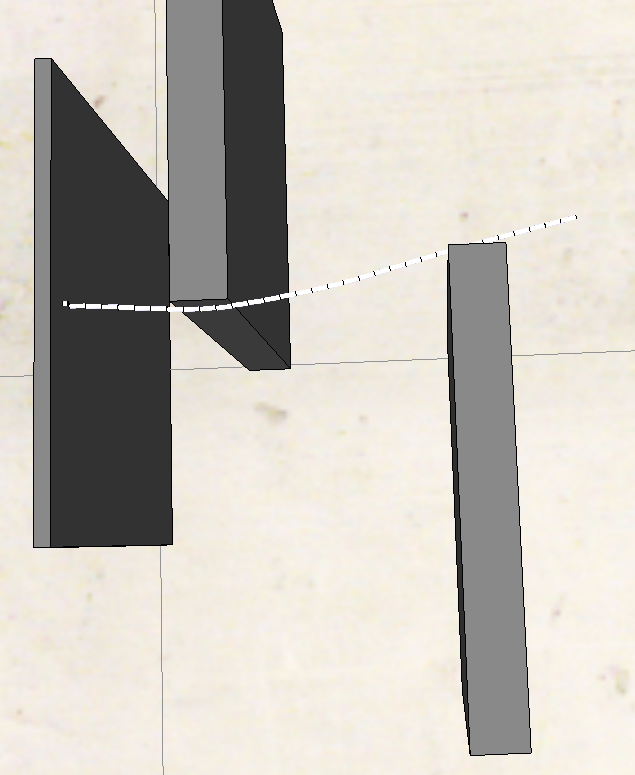
\includegraphics[width=\textwidth ,height=0.74\textwidth]{../force_experiment/exp6/vrep_photo.png}
		\caption{V-REP screenshot}
		\label{vrep_photo}
	\end{minipage}
\end{figure*}

Since we already discussed that by simply applying constant forces on the model resulted in a very unstable behavior of the catheter, we decide to apply multiple forces by creating a collision between world objects and the catheter. In this way we can create a deformation of the catheter which is also coherent with the experiments that we observed on the thesis. 

In practice, we used parallelepipeds that we translated on the plane in order to collide with the catheter model and apply a force. Then with the force sensor we can measure the actual force exerted on the model while knowing the contact points since we are posing the obstacle in such a way that it will only collide with a certain number of links. In this second trial, we applied a force on the link 27, 28 and 29 and the associated plots can be seen in the Figure: \ref{f_3_link}.
   
\subsection{6 Forces}

In the final experiment we use 2 parallelipeds in order to simulate contact points on different not adjacent points along the body of the catheter. In particular the forces were applied on the 7,8,9,10,25 and 26 links. The plots associated to the experiments can be seen in the Figure: \ref{f_6_link}, while in Figure: \ref{vrep_photo} we can see a screenshot of the V-REP environment when the catheter is beeing deformed.


\section*{Conclusions}

With this assignment we analyzed a new technique in order to estimate the contact forces along the body of a catheter which was modeled as a manipulator with elastic joints. Moreover, we tried to implement the proposed model in the V-REP simulation engine but several difficulties were encountered. Indeed, the complexity of the model can not be simulated in a correct way by the dynamic physic engine. This is mainly due to the large number of links that form the discretized catheter which can not be simulated in a proper way by the software. The bad behavior usually results in not negligible oscillations and vibrations in the structure which also influence the resultant of forces applied to it.

Still, several approaches were employed and an elasticity at the joint level can be actually developed by adjusting the control law that generates the commanded torque. Moreover, 1 DOF for each joint was the more stable solution for a simulation, while having 2 DOFs created too many vibrations in different directions.

Finally, we implemented the estimation method and saw that with our model the estimation usually is more accurate along the y direction while it is noisier along the x direction. But this might actually be due to the fact that given the instability of the model during the simulation we might depart too much from the static conditions and so a more dynamic setting should be considered. 

\begin{thebibliography}{9}

\bibitem{takashima}
K. Takashima, R. Shimomura, T. Kitou, H. Terada, K. Yoshinaka, and
K. Ikeuchi, \textit{“Contact and friction between catheter and blood vessel,”Tribology International}, vol. 40, no. 2, pp. 319–328, 2007.

\bibitem{khan}
F. Khan, R. J. Roesthuis, and S. Misra, “Force sensing in continuum manipulators using fiber bragg grating sensors,” in 2017 IEEE/RSJ \textit{International
Conference on Intelligent Robots and Systems (IROS)}. IEEE, 2017, pp. 2531–
2536.

\bibitem{khosnam}
M. Khoshnam, A. C. Skanes, and R. V. Patel, “Modeling and estimation of tip
contact force for steerable ablation catheters,” IEEE \textit{Transactions on Biomedical
Engineering}, vol. 62, no. 5, pp. 1404–1415, May 2015.

\bibitem{coppelia1}
Issue implementation flexible rope:
\\\textit{https://forum.coppeliarobotics.com/viewtopic.php?t=2665},
\\Coppelia member answer posted 18 Dec 2019, 23:33

\bibitem{spring}
Creating a Spring:
\\\textit{https://forum.coppeliarobotics.com/viewtopic.php?t=1307}

\end{thebibliography}

\end{document}